\section{Nuværende omkostninger i sundhedssektoren}
Det er relevant at se på omkostningerne i sundhedssektorens primære og sekundære sektor ved brug af den nuværende målemetode. 

\subsection{Primær sektor}
Den subjektive målemetode, der på nuværende tidspunkt benyttes af $27,7~\%$ af praktiserende læger, foregår ved spørgeskema under en konsultation, medfører udgifter i den primære sundhedssektor \citep{munck2007}. Afhængigt af antal konsultationer, som den enkelte kronikere har behov for, kan et spørgeskema følge med hver konsultation, og omkostningerne til denne målemetode vil derved stige. Udarbejdelse og udskrifter af et spørgeskema vil have relativt lave omkostninger.
\citeauthor{munck2007} udarbejdede i 2007 en rapport om hypertension i almen praksis. Her blev 159 kontaktpersoner i almen praksis spurgt: "Sætter I jeres hypertensionspatienter til kontrol med fast tidsinterval? Hvis ja, angiv det typiske interval". Her svarede $92,5~\%$, at de sætter deres patienter til kontrol med et fast tidsinterval, og i gennemsnit er dette interval udregnet til 3,9 måneder \citep{munck2007}. 

Hvis det, jævnfør \citeauthor{kronborg2008}, antages at $1/5$ af den voksne danske befolkning har hypertension, vil dette svare til omkring 900.000 danskere \citep{folketal2016}. Hvis 900.000 danskere skal til lægekonsultation á 137,93 kroner hver 3,9. måned, vil dette svare til en årsomkostning for sundhedssektoren på omkring 380 millioner kroner \citep{honorartabel2016}. 

Den samlede medicinudgift i den primære sundhedssektor i Danmark i 2014 lå på 11,6 milliarder kroner, og Danmarks Statistik påpeger i denne sammenhæng, at blodtrykssænkende medicin og hjertemedicin er nogle af de mest anvendte former for medicin i Danmark \citep{dst2016}. 

\subsection{Sekundær sektor}
Den sekundære sektor påvirkes også af hypertension på den måde, at sygdommen er skyld i ambulante besøg og indlæggelser. I 2014 var der $49.875$ ambulante besøg i den offentlige sekundære sektor for patienter med diagnosen blodtryksforhøjelse af ukendt årsag eller blodtryksforhøjelse af kendt årsag, hvilket svarer til en stigning på $8,35~\%$ siden 2012, hvilket kan ses på \autoref{fig:hyp_sekundaer} \citep{sundhedsdatastyrelsen2016}. 

\begin{figure}[H]
\centering
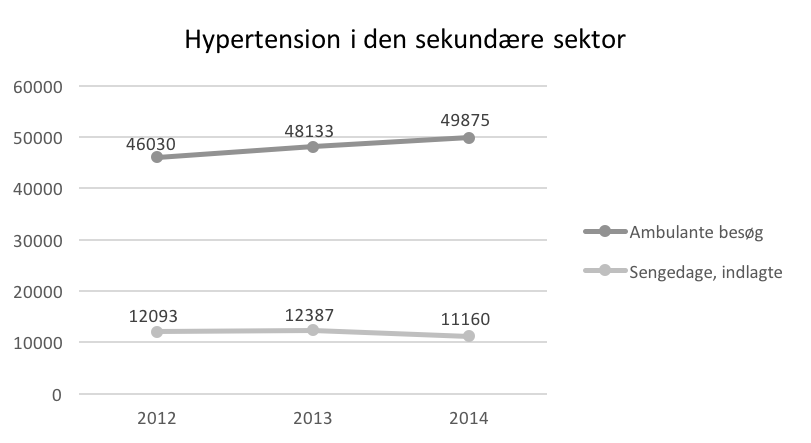
\includegraphics[width=0.8\textwidth]{figures/hyp_sekundaer}
\caption{Henvendelser i den offentlige sekundære sektor som følge af hypertension fra 2012 til 2014 \citep{sundhedsdatastyrelsen2016}.}
\label{fig:hyp_sekundaer}
\end{figure}

\noindent
Yderligere havde patienter med hypertension $11.160$ sengedage i forbindelse med indlæggelse på offentlige sygehuse i 2014, hvilket var et fald i forholdt til de to foregående år \citep{sundhedsdatastyrelsen2016}. 